\documentclass[pdf]{beamer}
\mode<presentation> {
   \usetheme{Warsaw}
}

\usepackage[english]{babel}
\usepackage[utf8]{inputenc}
\usepackage{beamerprosper}
\usepackage{graphicx}
\usepackage{colortbl}
\usepackage{wrapfig}
\usepackage{subfig}
\usepackage{tikz}

\providecommand{\uv}[1]{\quotedblbase #1\textquotedblleft}
\providecommand\bi{\begin{itemize}}
\providecommand\ei{\end{itemize}}
\providecommand\li{\item}

\addtobeamertemplate{footline}{
  \setbeamertemplate{footline}[page number]
  \setbeamercolor{page number in head/foot}{use=headline,fg=headline.fg,bg=headline.bg}
  \usebeamertemplate{footline}
}{}

\definecolor{mylightblue}{rgb}{0.5,0.5,0.90}
\definecolor{highlight}{rgb}{1,1,0.5}


\begin{document}
	\usenavigationsymbolstemplate{}
	\title {Automatic calibraton of the camera with Velodyne LiDAR}
	\institute{Michal Spanel (supervisor), Zdenek Materna (HW)\\\medskip
	Department of Computer Graphics and Multimedia FIT BUT \\\smallskip\texttt{\scriptsize ivelas@fit.vutbr.cz}}
	\author {Martin Velas}
	\begin{frame}
		\titlepage
	\end{frame}
	
	\begin{frame}{Motivation}
 		\begin{block}{Usage of the fusion}
			\begin{itemize}
				\item coloured point cloud (depth $+$ color)
				\item description of the $3$D points by the image features
				\item sensors must be calibrated
			\end{itemize}
		\end{block}

		\begin{itemize}
			\item position and orientation of LiDAR to the camera ($6$DoF)
			\item $\Rightarrow$ calibration matrix (rotation $+$ translation)
		\end{itemize}
		
		\begin{figure}[h]
			\center
			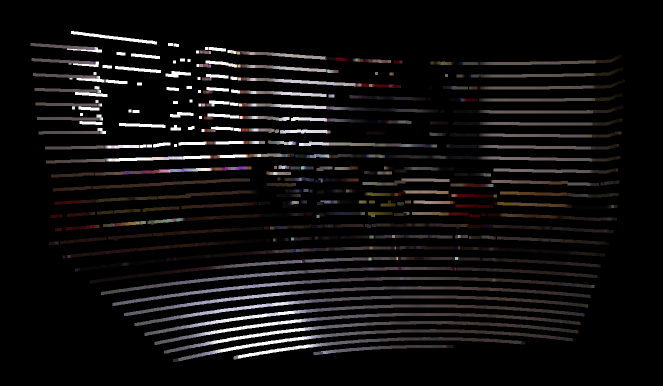
\includegraphics[width=0.55\textwidth]{fig/colored_cloud.png}
		\end{figure}
			
	\end{frame}
	
	\begin{frame}{Used sensors}
		\begin{itemize}
			\item RGB camera of Kinect (depth map not used)
			\item \emph{Velodyne} LiDAR (laser radar)
			\begin{itemize}
				\item $360^{\circ}$ horizontal and $-10^{\circ}$ to $+30^{\circ}$ vertical field of view
				\item beam rotates $10$ times per sec 				
				\item $32$/$64$ rays (depends on the model) each capturing the $3$D points of one "ring"
				\item $700\,000$ points captured per second
			\end{itemize}
		\end{itemize}	
		\begin{figure}[h]
			\center
			\subfloat{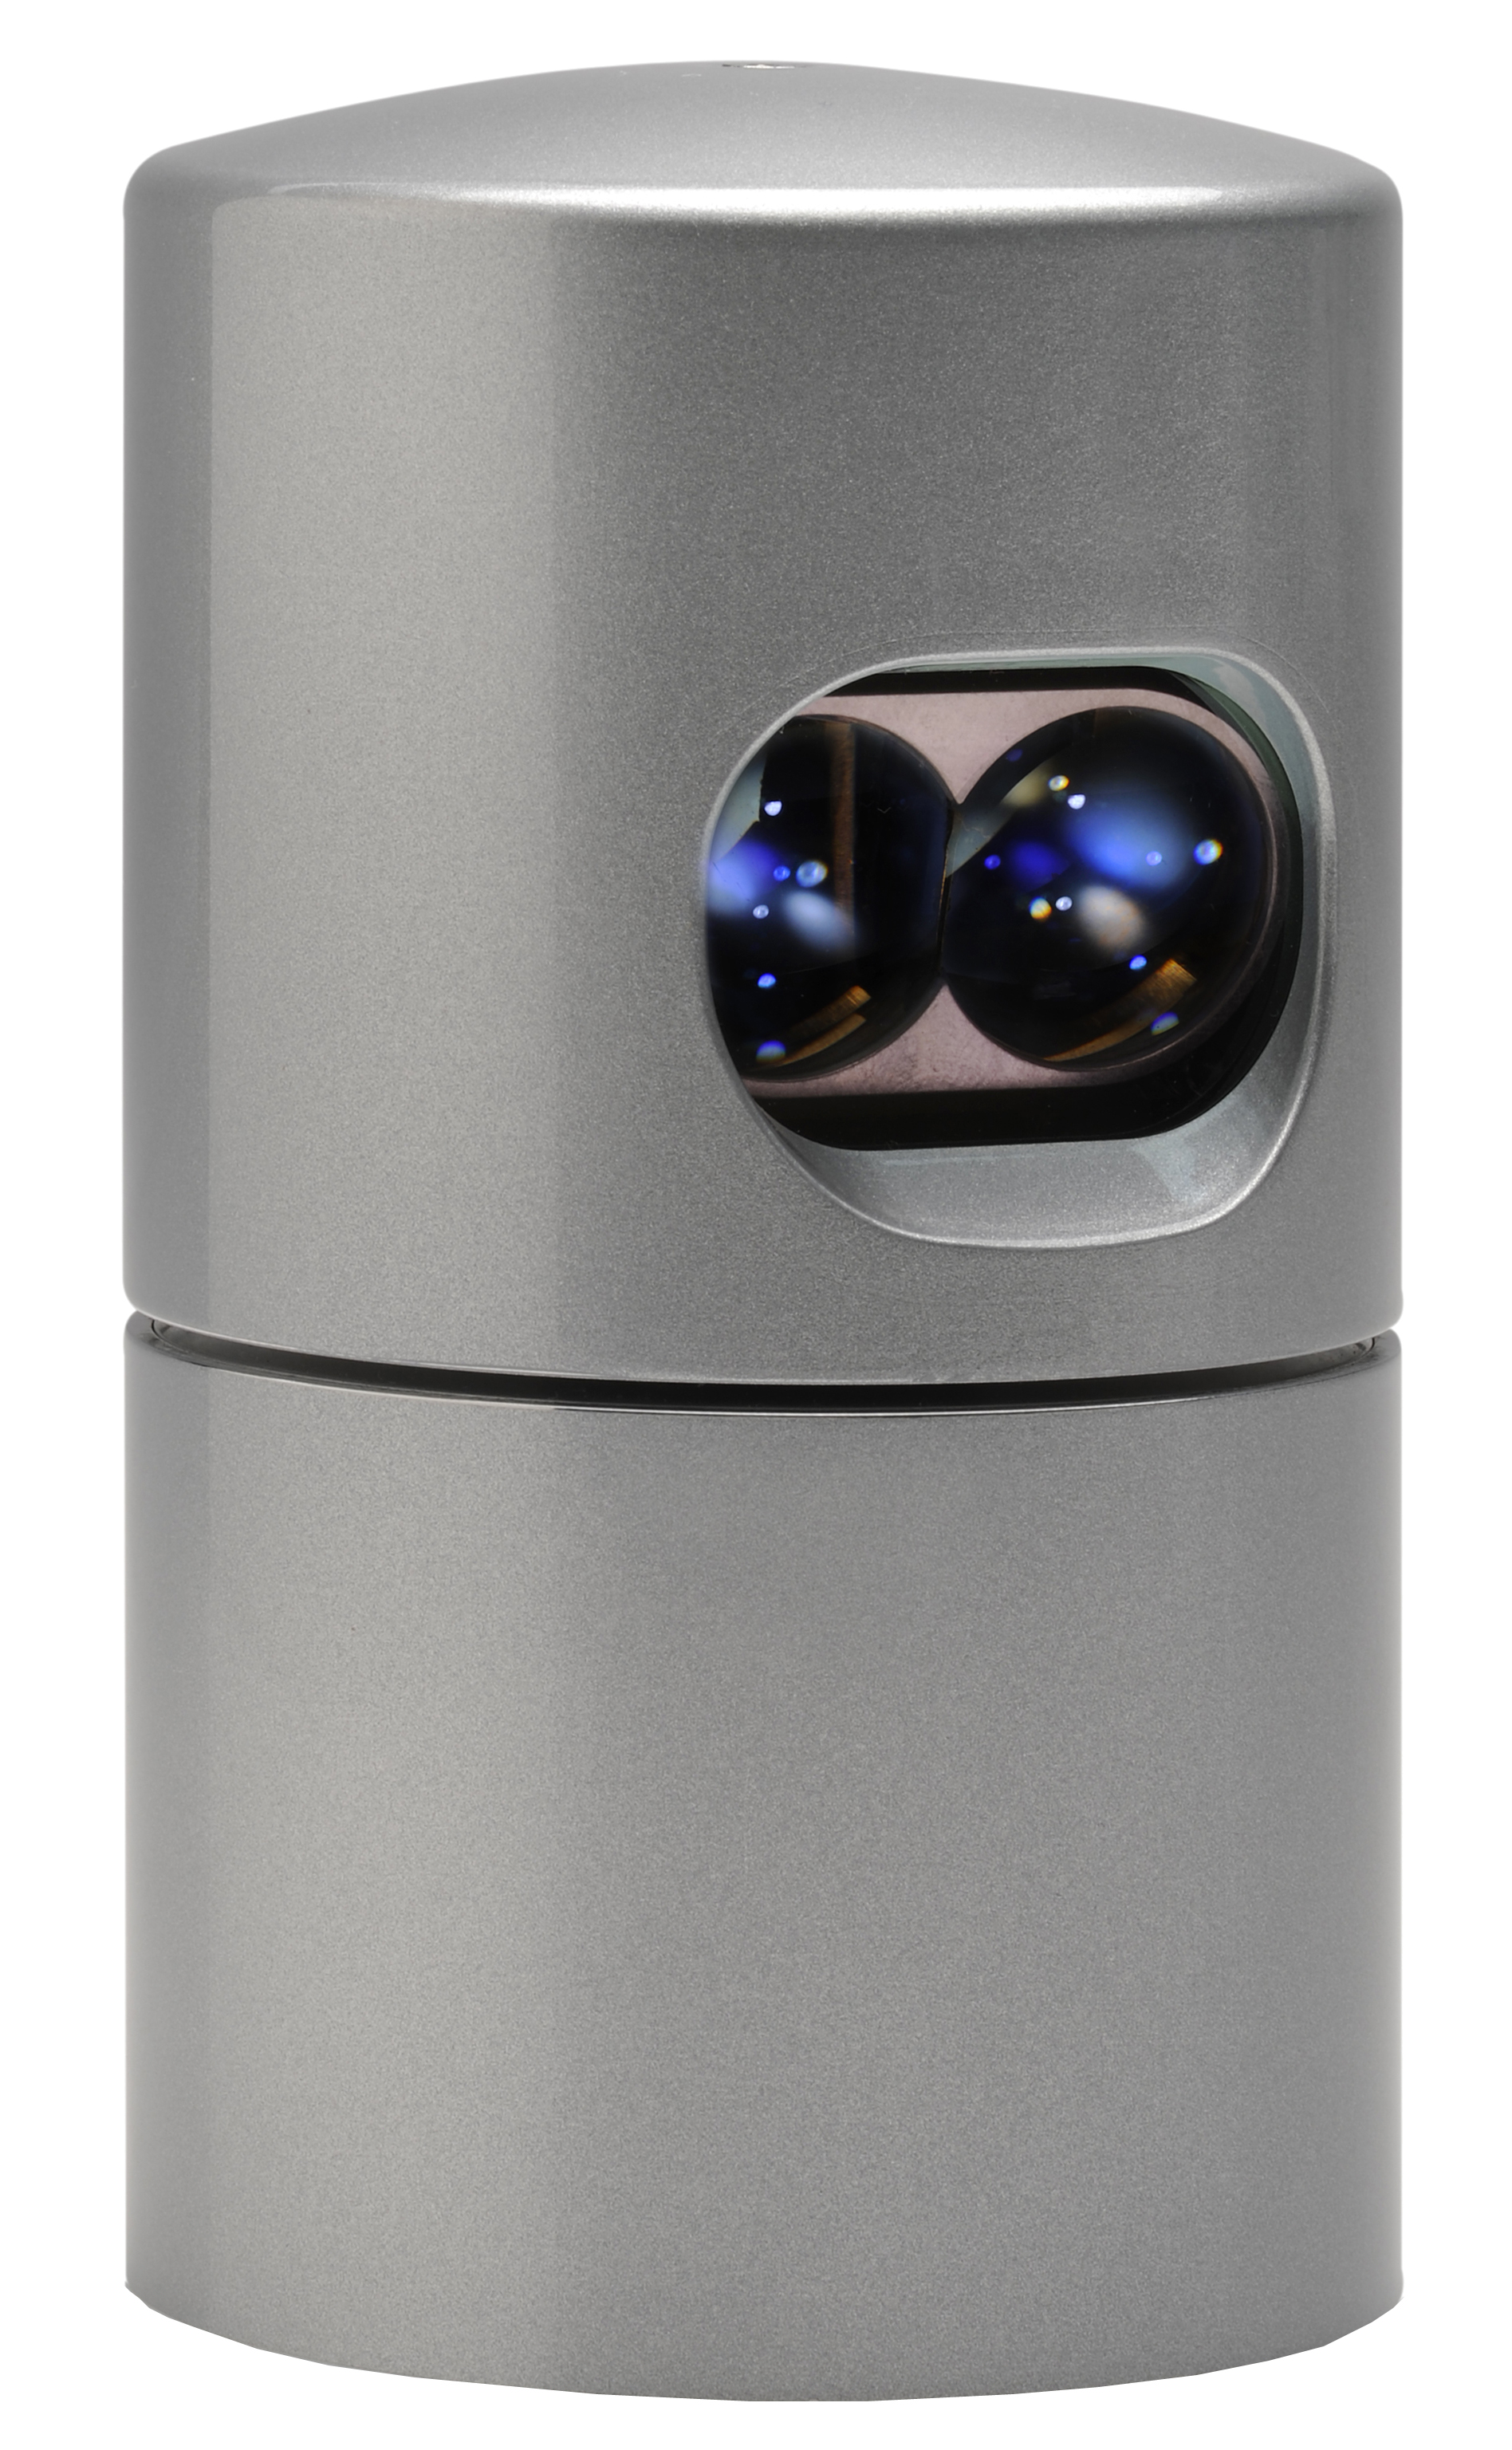
\includegraphics[height=0.35\textwidth]{fig/velodyne_32.png}}
			\quad
			\subfloat{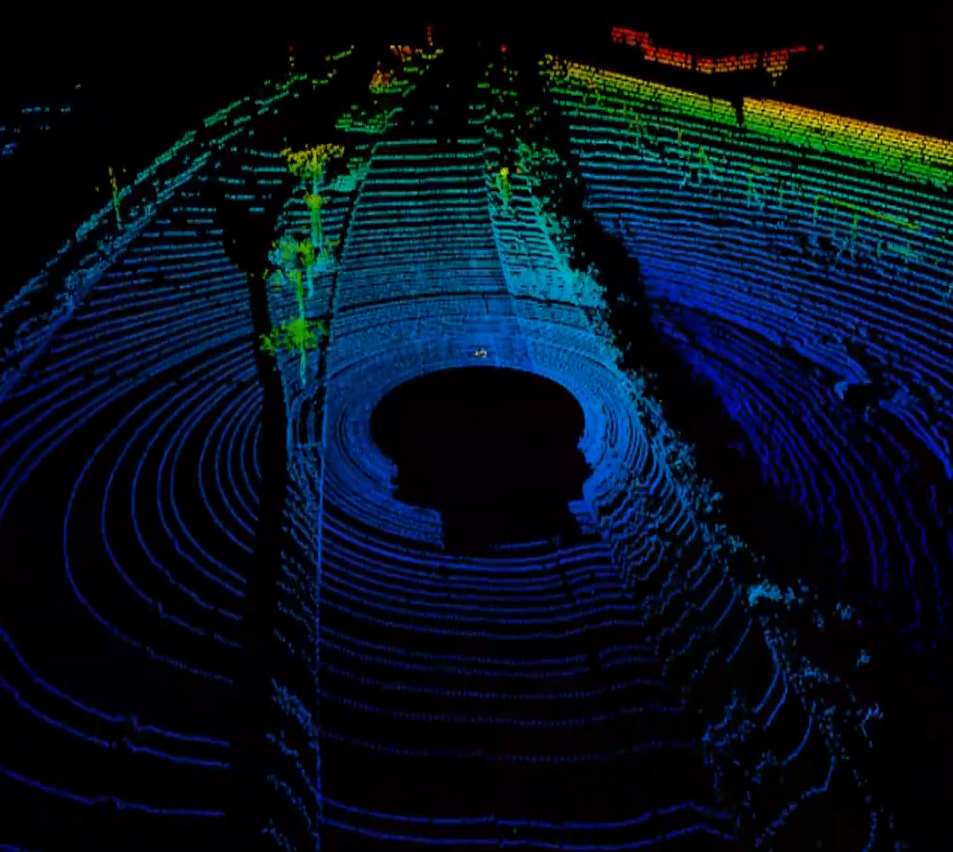
\includegraphics[height=0.35\textwidth]{fig/velodyne_scan.png}}
			\quad
			\subfloat{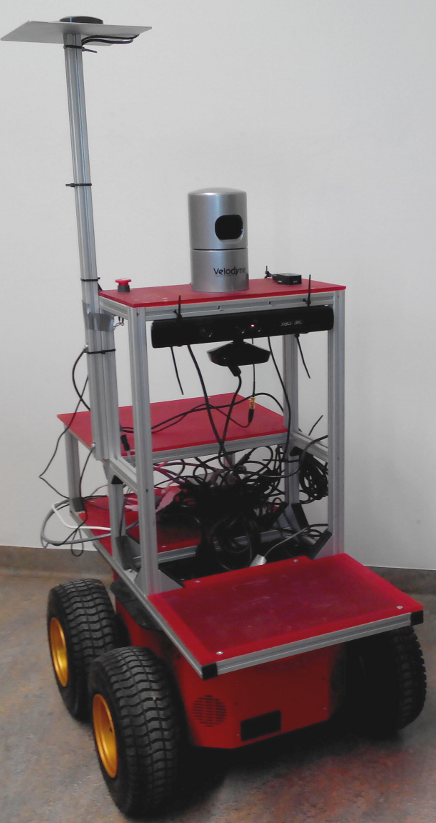
\includegraphics[height=0.35\textwidth]{fig/robot.png}}
		\end{figure}
	\end{frame}
	
	\begin{frame}{Edge detection}
		\begin{alertblock}{Assumption (proved)}		
		\begin{itemize}
			\item edges can be robustly detected in both camera image and Velodyne scan
			\item \scriptsize{Levinson, J.; Thrun, S.: Automatic Online Calibration of Cameras and Lasers}
		\end{itemize}
		\end{alertblock}
		
		\begin{itemize}
			\item in edge image by the Sobel operator
			\item in the Velodyne LiDAR scan (point cloud) as the depth discontinuities of the neighbouring points in the ring
			\begin{equation}
				X_i = max(P_{i-1}.r - P_i.r, P_{i+1}.r - P_i.r, 0)^\gamma
			\end{equation}
		\end{itemize}
	\end{frame}

	\begin{frame}{Calibration pipeline}
		\begin{enumerate}
			\item \emph{Coarse calibration}
			\begin{enumerate}
				\item edge detection in the Velodyne point cloud and the camera image
				\item $3$D marker detection (circles' centres and the radius)
				\begin{enumerate}
					\item in the camera image using the Hough transform
					\item in the point cloud using the proposed detection algorithm
				\end{enumerate}
				\item geometrical transformation between sensors estimation (translation only)
			\end{enumerate}
			\item \emph{Calibration refinement}
			\begin{enumerate}
				\item dense search in the small subspace of calibration parameters
				\item pick the calibration solution based on the proposed criteria
			\end{enumerate}
		\end{enumerate}
	\end{frame}

	\begin{frame}{Coarse calibration -- marker selection}
		\setcounter{subfigure}{0}
		\begin{figure}[h]
			\centering
			\subfloat[][]{
			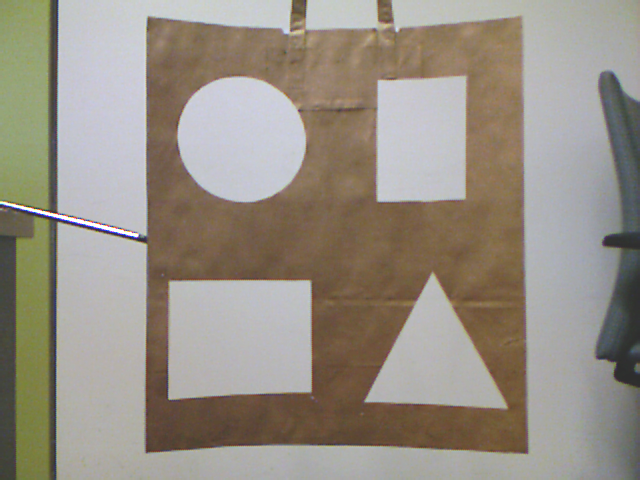
\includegraphics[width=0.35\textwidth]{fig/geom-shapes-all-img.png}}
			\quad
			\subfloat[][]{
			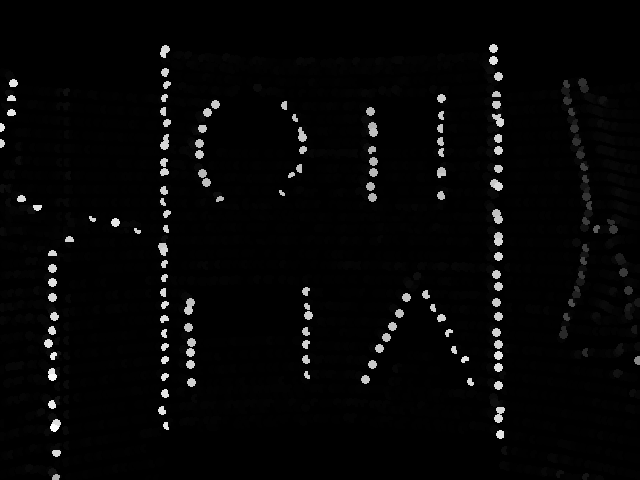
\includegraphics[width=0.35\textwidth]{fig/geom-shapes-all-velodyne.png}}
			
			\medskip\medskip\medskip		
			
			\subfloat[][]{
			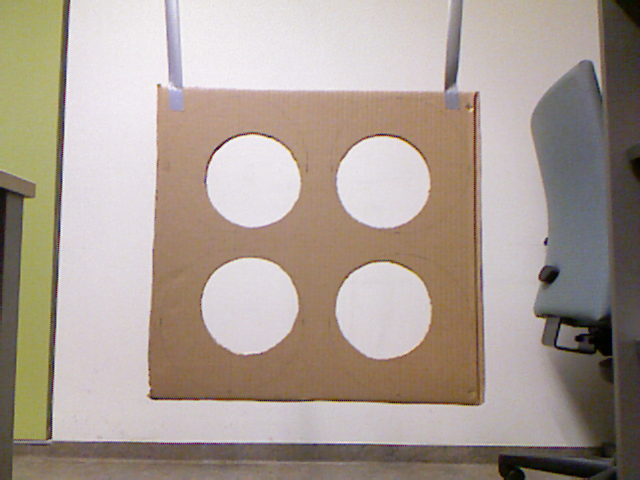
\includegraphics[width=0.35\textwidth]{fig/geom-shapes-circles-img.png}}
			\quad
			\subfloat[][]{
			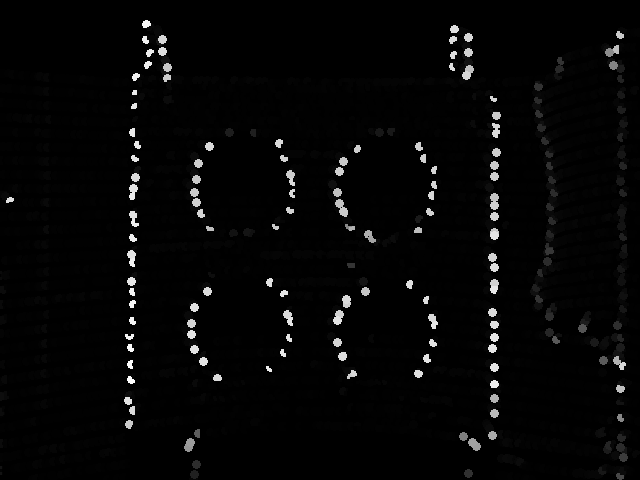
\includegraphics[width=0.35\textwidth]{fig/geom-shapes-circles-velodyne.png}}
		\end{figure}
	\end{frame}

	\begin{frame}{Coarse calibration -- marker detection}
		\begin{itemize}
			\item in \emph{camera image}
			\begin{itemize}
				\item Sobel edge detection $+$ Hough transform
				\item easy-peasy-lemon-squeezy and robust enough
			\end{itemize}
			\item in \emph{Velodyne point-cloud} (proposed algorithm)
			\begin{enumerate}
				\item edge detection
				\item thresholding (mass point reduction $10k \rightarrow 100$)
				\item detect $4$ spheres intersecting the plane \label{step:detection}
				\item verification
				\item if fails the candidates generation and goto \ref{step:detection}
			\end{enumerate}
		\end{itemize}
	\end{frame}

	\begin{frame}{Coarse calibration -- translation computing}
		\begin{itemize}
			\item we assume
			\begin{itemize}
				\item translation is more significant than rotation
				\item marker is planar object
			\end{itemize}
			
			\item we know intrinsic parameters 
			\begin{itemize}
				\item focal length $f$ and the principal point $[o_x, o_y]$
			\end{itemize}
			
			\item we have the correspondences
			\begin{itemize}
				\item 3$D$ point $[X, Y, Z] \rightarrow 2$D point $[x, y]$ (circles centres)
				\item and radiuses $r_{3D} \rightarrow r_{2D}$ of the circles (from image/point-cloud)
			\end{itemize} 
		\end{itemize}
		\begin{eqnarray}
			t_z =& \dfrac{r_{3D}.f}{r_{2D} - Z} \\
			t_x =& \dfrac{(x - o_x).(Z + t_z)}{f} - X   \\
			t_y =& \dfrac{(y - o_y).(Z + t_z)}{f} - Y
		\end{eqnarray}
	\end{frame}
	
	\begin{frame}{Fine calibration}
		\begin{figure}[h]
			\center
			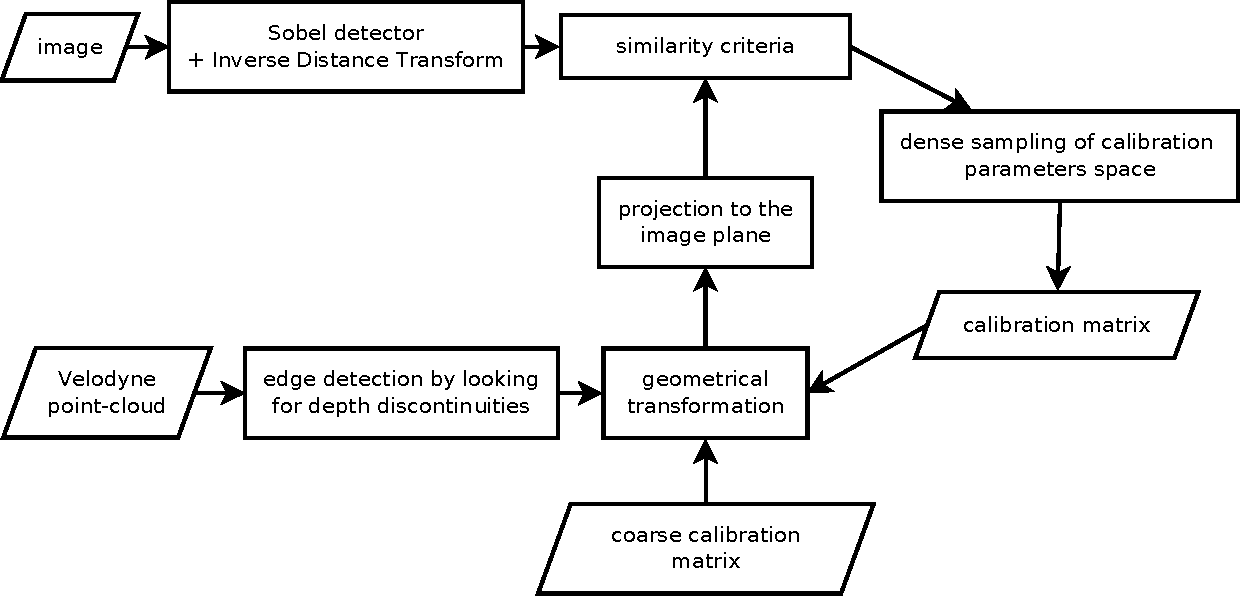
\includegraphics[width=0.99\textwidth]{fig/framework.pdf}
		\end{figure}
		\begin{itemize}
			\item based on the [Levin09] $+$ modifications
		\end{itemize}
	\end{frame}	

	\begin{frame}{Similarity criteria}
		\begin{itemize}
			\item \emph{Inversed Distance Transform (IDT)} makes both edge image and the similarity criteria ``smoother''
			$$
				D_{i,j} = \alpha . E_{i,j} + (1-\alpha)\,.\,\underset{x,y}{max}\{ E_{x,y} . \gamma^{max(\vert x-i \vert, \vert y-j \vert)}\}
			$$
			\begin{figure}[h]
				\center
				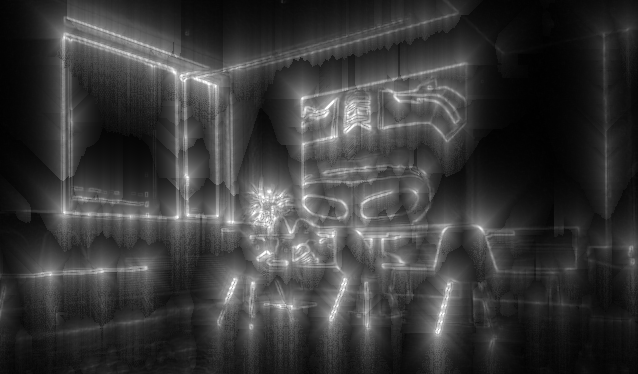
\includegraphics[width=0.4\textwidth]{fig/edges_idt.png}
			\end{figure}
			\item \emph{edge based criteria} -- cross correlation of IDT image with projected $3$D points
		\end{itemize}
		
		\begin{block}{Novel \emph{projection error criteria}}
			\begin{itemize}
				\item scene segmentation (foreground/background)
				\item percentage of miss-projected $3$D points
			\end{itemize}
		\end{block}
	
	\end{frame}
	
	\begin{frame}{Results -- coarse calibration (vs. manual)}
		\begin{figure}[h!]
			\centering
			\subfloat{
			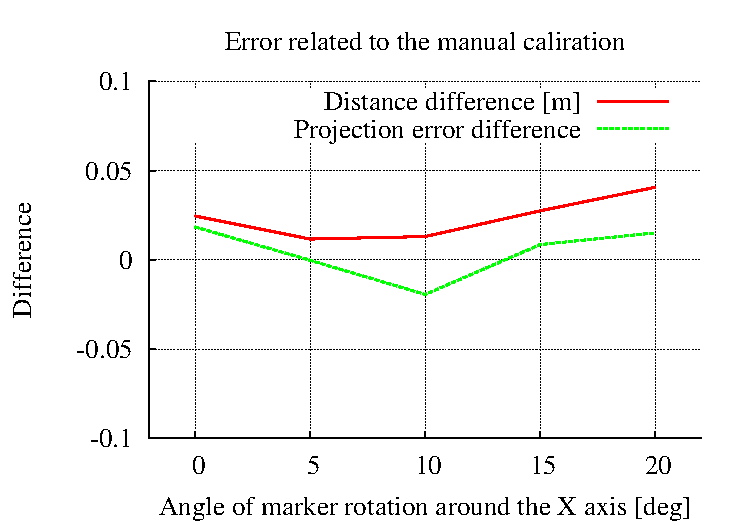
\includegraphics[width=0.45\textwidth]{fig/results-x.pdf}}
			\subfloat{
			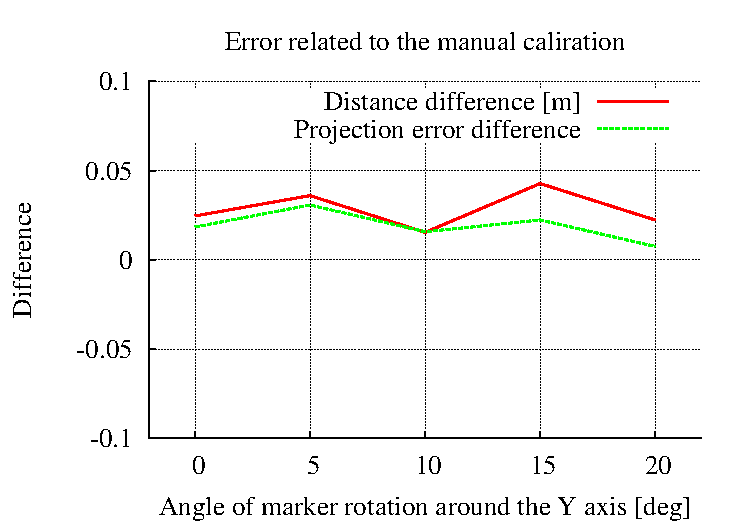
\includegraphics[width=0.45\textwidth]{fig/results-y.pdf}}
			
			\subfloat{
			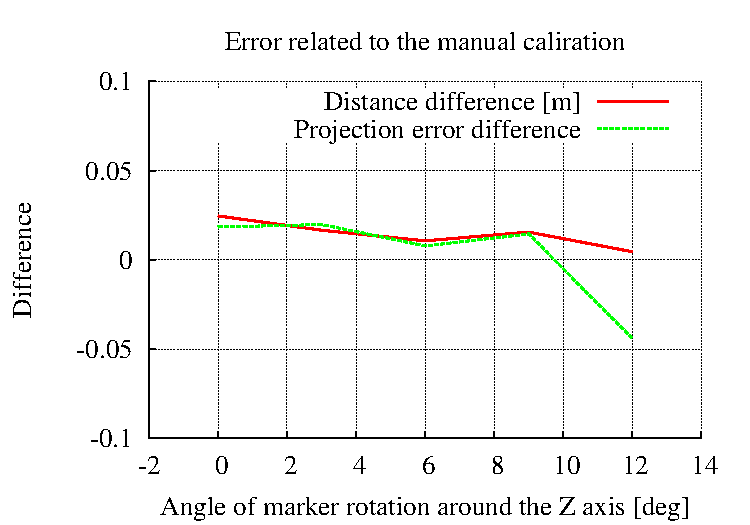
\includegraphics[width=0.45\textwidth]{fig/results-z.pdf}}
			
		\end{figure}
	\end{frame}	
	
	\begin{frame}{Results -- fine calibration}
		\newcommand\minus{%
		  \setbox0=\hbox{-}%
		  \vcenter{%
		    \hrule width\wd0 height \the\fontdimen8\textfont3%
		  }\,%
		}
		\begin{table}[h]
			\centering
			\begin{tabular}{|l|l|l|l|}
				\hline
				 & $\vec{t}\, ;\,\, \vec{r}$ &   $S_E$ & $E_P$  \\
				\hline\hline
				
				Manual & $[0.006, \minus 0.089, \minus 0.1];$ & $3.29$ & $0.112$ \\
				& $[0,0,0]$ & & \\
				\hline
				Coarse & $[0.002, \minus 0.098, \minus 0.13]$ & $3.13$ & $0.141$ \\
				& $[0,0,0]$ & & \\
				\hline
				[Levin09] & $[0.022, \minus 0.118, \minus 0.11]$ & $3.35$ & $0.193$ \\
				& $[\minus 0.005, 0.01, 0]$ & & \\
				\hline
				[Levin09] & $[0.003, \minus 0.1, \minus 0.13]$ & $3.16$ & $0.140$ \\
				+Avg.& $[2.10^{\minus 4}, 0, 0]$ & & \\
				\hline
				Projection & $0.002, \minus 0.088, \minus 0.11$ & $3.26$ & $0.111$ \\
				& $[0.005, 0, 0]$ & & \\
				\hline
				
			\end{tabular}
		\end{table}
		
		\begin{itemize}
			\item $S_E$ -- similarity criteria based on the edges
			\item $E_P$ -- projection error
		\end{itemize}
	\end{frame}	
	
	\begin{frame}{Results -- visual comparison}
		\setcounter{subfigure}{0}
		\begin{figure}[htb]
			\centering
			\subfloat[a][Coarse]{
			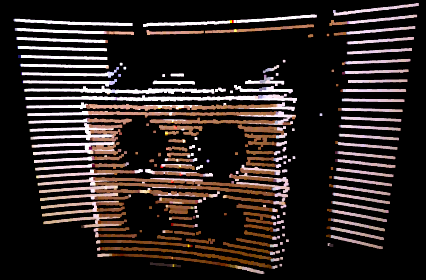
\includegraphics[width=0.40\textwidth]{fig/coarse-c.png}}
			\subfloat[b][Levin09]{
			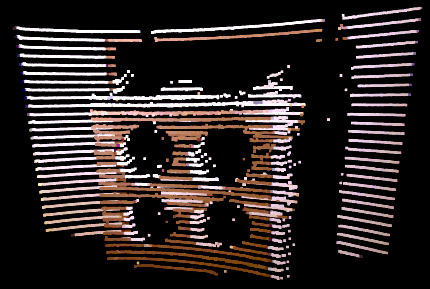
\includegraphics[width=0.40\textwidth]{fig/levin-c.png}}
			\\
			\subfloat[c][Levin09+Avg.]{
			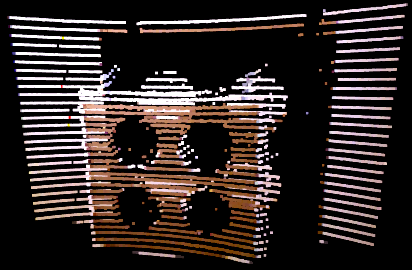
\includegraphics[width=0.40\textwidth]{fig/levin-avg-c.png}}
			\subfloat[d][Projection error]{
			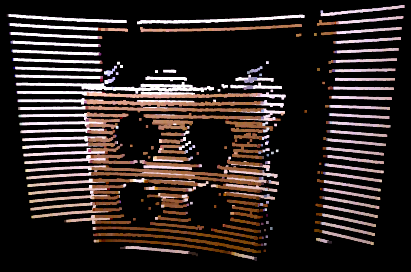
\includegraphics[width=0.40\textwidth]{fig/project-c.png}}
		\end{figure}
	\end{frame}
	
\end{document}
